\documentclass[letterpaper,twocolumn,10pt]{article}
\usepackage{epsfig,xspace,url}
\usepackage{authblk}
\usepackage{graphicx}
\graphicspath{ {images/} }

\title{Third Party Encrypted Storage}
\author{Travis Taylor, John Robe, and Daniel James}
\affil{School of Computing, University of Utah}

\begin{document}

\maketitle

\section{Introduction}

\section{Design}

Add basic idea here

See figure \ref{design}.

Our basic design consists of four entities
\begin{itemize}
    \item \textbf{User} - The user that desires to use our application, to store their data securely
    \item \textbf{Authentication Server} - The server that will store the encrypted data for the user, without having the key.
    \item \textbf{Portal Application} - This is the application that retrieves data from the user to unlock the data on the authentication server.
    \item \textbf{Demo Application} - This application is the entity that requests data about the user.
\end{itemize}

\begin{figure*}[ht]
\centering
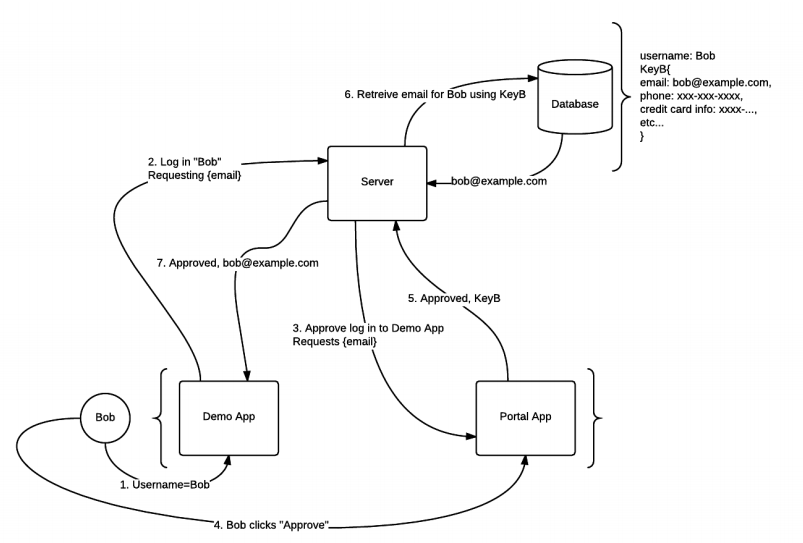
\includegraphics[width=\textwidth]{Design}
\caption{Overall system design}
\label{design}
\end{figure*}



\section{Implemention}
%TODO Probably add more here between the example run through and the first sentence
    We chose to write our demo application in three parts: the server, the portal, and the demo application. An example run through of our application would like like so:
\begin{figure}[ht]
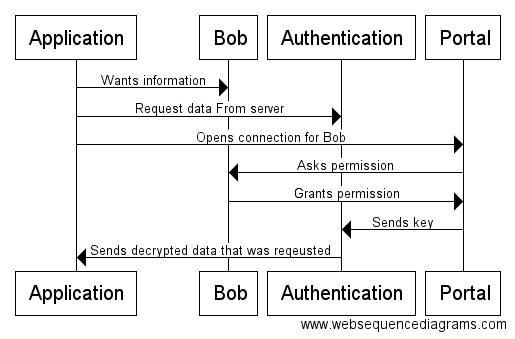
\includegraphics[width=0.45\textwidth]{messageDiagram}
\caption{Message Flow}
\end{figure}

\subsection{Authentication Server}
    The authentication server deals with holding the encrypted data. It is relatively simple, as it merely has to hold a 2 column table, and provide the ability to decrypt with a given key. The server provides this functionality through Apache Thrift\cite{thrift}. It provides some simple functions:
    \begin{itemize}
        \item \textbf{createAccount} - Creates the account for the user, and generates the key for it.
        \item \textbf{requestPermission} - The application requesting access will call this function with the requested data fields and user.
        \item \textbf{checkForPermissionRequest} - Portal can check if it has any pending reqeusts\footnote{In lieu of push notifications, we moved for polling due to time constraints} 
        \item \textbf{decideRequest} - Once the user decides what they want to do, the portal application will call this with the decision and, if in the affirmative, the key.
        \item \textbf{checkForPermissionGranted} - The demo application can poll with a requerst ID to see if their request has been confirmed or denied.
    \end{itemize}

The backend storage is SQLite, given the simple nature of the data.
\subsection{Portal Application}
\subsection{Demo Application}

\section{Alterative Methods}


{
    \small
    \bibliographystyle{acm}
    \bibliography{biblio}
}

\end{document}
